\documentclass[5pt]{article}
\usepackage{multicol,multirow}
\usepackage{graphicx} % Required for inserting images
\usepackage[margin=0.75cm]{geometry}
\usepackage{xcolor}
\usepackage{amsmath,esint}
\usepackage{mathtools}
\usepackage{relsize}
\usepackage{mathtools}
\usepackage{nccmath}
\usepackage[inline]{enumitem}
\usepackage{algpseudocode}

\usepackage{empheq}
\usepackage{amsfonts}

\usepackage{tkz-euclide}
\usepackage{tikz}

\definecolor{LightGray}{gray}{0.9}

\usepackage{minted}

\newenvironment{amatrix}[1]{%
  \left[\begin{array}{@{}*{#1}{c}|c@{}}
}{%
  \end{array}\right]
}

\DeclarePairedDelimiter\abs{\lvert}{\rvert}%
\DeclarePairedDelimiter\norm{\lVert}{\rVert}%
\newcommand{\universalSet}{\mathbb{U}}

\makeatletter
\let\oldabs\abs
\def\abs{\@ifstar{\oldabs}{\oldabs*}}

\newcommand{\tr}[3]{
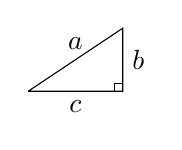
\begin{tikzpicture}[scale=0.40]
    \coordinate [] (A) at (-1.5cm,-1.cm);
    \coordinate [] (C) at (1.5cm,-1.0cm);
    \coordinate [] (B) at (1.5cm,1.0cm);
    \draw (A) -- node[above] {$a$} (B) -- node[right] {$b$} (C) -- node[below] {$c$} (A);
    \draw (1.25cm,-1.0cm) rectangle (1.5cm,-0.75cm);
\end{tikzpicture}
}


\begin{document}
\newtheorem{theorem}{Theorem}


\begin{center}
     \Large{\textbf{Discrete Mathematics}}\\
     \small{Class: MATH 2410}\hfill\small{\textcopyright Maximilien Notz \the\year{}}
     \noindent\rule{20.2cm}{0.4pt}
\end{center}


\begin{multicols}{2}
\setcounter{secnumdepth}{0}

\subsection{Mathematical Statement}
\begin{tabular}{ll}
    Statement       & is any declarative sentence which is either true\\
                    & or false.\\
    Atomic          & if it cannot be divided into smaller statements.\\
    Molecular       & if it can be divided into smaller statements.\\
    conjunction     & $p\land q$ equivalent to "$p$ and $q$".\\
    disjunction     & $p\lor q$ equivalent to "$p$ or $q$".\\
                    & where $p$ is the hypothesis and $q$ the conclusion.\\
    Implication     & $p\rightarrow q$ equivalent to "if $p$ then $q$".\\
    Biconditional   & $p\leftrightarrow q$ equivalent to "if and only if $p$ then $q$".\\
    Negation        & $\lnot p$ equivalent to "not $p$".\\
    Converse        & \\
    Contrapositive  & \\
    There is a $x$  & $\exists x$\\
    For all $x$     & $\forall x$\\
    
    
\end{tabular}

\subsection{Naive Set Theory}
\subsubsection{Set Notation}
\begin{tabular}{ll}
    Universal set           & $\universalSet$\\
    Empty set               & $\emptyset=\{\}$, Remember: $\forall A (\emptyset\subset A)$\\
    Power set               & $\mathcal{P}(A)$ is the set of all the subsets of $A$.\\
    Partition of $A$        & A collection of nonempty, \small{pairwise-disjoint}\\
                            & subsets whose union is $A$.\\
    Element of              & $\in$. Example:$2\in\{1,2,3\}$\\
    Subset of               & $\subseteq$. Example: $\{A, B,C\}\subseteq\{B,C,D\}$\\
                            & $A\subseteq B \Leftrightarrow\forall x$\\
    Proper subset of        & $\subset$. Example: $\{A, B,C\}\subset\{A, B,C,D\}$\\
    Intersection            & $\bigcap_{i\in I}A_i=\{x\in\universalSet|\forall i\in I, x\in A_i\}$\\
                            & $A\cap B=\{x\in\universalSet|x\in A\land x\in B\}$\\
    Union                   & $\bigcup_{i\in I}A_i=\{x\in\universalSet|\exists i\in I, x\in A_i\}$\\
                            & $A\cup B=\{x\in\universalSet|x\in A\lor x\in B\}$\\
    Difference              & $A\backslash B=\{x\in A|x\notin B\}$\\
    Symmetric difference    & $A\Delta B=(A\backslash B)\cup(B\backslash A)$\\
    Cartesian Product       & $A\times B=\{(x,y)|x\in A\land y \in B\}$\\
    Complement of           & $\bar{A}=\{x\in\universalSet|x\notin A\}$\\
    Cardinality             & $|A|$
    
\end{tabular}

\subsubsection{Cardinality}
\begin{tabular}{ll}
    finite set      & Let $X$ be a finite set then $|X|\in \mathbb{N}$\\
    countable set   & A set $S$ is countable if and only if that is finit\\
                    & or $|S|=|\mathbb{N}|$.\\
    aleph null.     & $\aleph_0=|\mathbb{N}|$\\
\end{tabular}

\begin{theorem}
    Let $A$ and $B$ be sets, then $|A|=|B|$ if and only if there is a one-to-one correspondence from $A$ to $B$.
\end{theorem}

\begin{theorem}
    If $A$ and $B$ are countable, then $A\cup B$ is countable. 
\end{theorem}

\begin{theorem}[Cantor's Theorem]
    For every set $A$, $|A|<|\mathcal{P}(A)|$.
\end{theorem}

\begin{theorem}[Schr\"oder--Bernstein]
     If there are injective function(one-to-one) functions $f\!:A\to B$ and $g\!:B\to A$, then there is a one-to-one correspondence between $A$ and $B$. 
     In other words If $A$ and $B$ are set with $|A|\neq|B|$ and $|B|\neq|A|$, then $|A|=|B|$.
\end{theorem}

\subsection{Functions}

\begin{tabular}{ll}
    Functions           & A rule that assigns each input exactly one \\
                        & output.\\
    Domain              & The set of all input of a function.($X$ in $f:X\rightarrow Y$)\\
    Codomain            & The set of all output a function.($Y$ in $f:X\rightarrow Y$)\\
    Range               & Is the subset of Y of elements that have an\\
                        & antecedent in X by f\\
    $f:x\rightarrow y$  & a function $f$ with a domain $x$ and a codomain $y$.\\
    Recursive f.        & \\
    Injective           & every element of the codomain is the image  of \\
                        & $f(a)=f(b)\Rightarrow a=b$\\
                        & \textbf{at most} one element from the domain.\\
    Surjective          & every element of the codomain is the image  of \\
                        & \textbf{at least} one element from the domain.\\
    Bijection           & A function that is \textbf{Injective} and \textbf{Surjective}.\\
    Image               & $f(A)=\{f(a)\in Y: a\in A\}$, where $A\subset\text{domain}$.\\
    Inverse Image       & $f^{-1}(B)=\{f(b)\in X: b\in B\}$, where \\
                        & $B\subset\text{codomain}$.\\
\end{tabular}

\subsection{Counting}

\begin{tabular}{ll}
    power set cardinality   & $|\mathcal{P}(A)|=2^{|A|}$\\
    n-bit string            & \\
    bit string weight       & the number of \textbf{1} in a bit string.\\
    $B^n_k$                 & the set of all \textbf{n-bit strings} of weight k.\\
\end{tabular}

\subsubsection{Additive Principle}
\textbf{General Definition:} 
if event $A$ can occur in $m$ ways, and even $B$ can occur in $n$ \textbf{disjoint} ($A$ and $B$ can't apen at the same time.) ways, then $A$ and $B$ can occur in $m+n$ ways.\\   
\textbf{Set Definition:} Given 2 sets $A$ and $B$, if $A\cap B =\emptyset$, then $|A\cap B| = |A| + |B|$.


\subsubsection{Multiplicative Principle}
\textbf{General Definition:} if event $A$ can occur $m$ ways, and each possibility for $A$ allows for exactly $n$ ways for event $B$, then the event "$A$ and $B$" can occur $m\cdot n$ ways.\\
\textbf{Set Definition:} Given 2 sets $A$ and $B$, we have $|A\times B|=|A|\cdot|B|$.

\subsubsection{Binomial coefficient}

\subsection{Sequences}

\subsection{Symbolic Logic}
\subsubsection{deMorganLaws}
\begin{itemize*}
    \item $\lnot\forall xP(x)=\exists xp(x)$
    \item $\lnot\exists xP(x)=\forall xp(x)$
    \item $\lnot(a_1\land a_2\land \dots\land a_n)\equiv \lnot a_1\lor \lnot a_2\lor \dots\lor \lnot a_n$
    \item $\lnot(a_1\lor a_2\lor \dots\lor a_n)\equiv \lnot a_1\land \lnot a_2\land \dots\land \lnot a_n$
\end{itemize*}


\subsection{Proofs}

\subsection{Graph Theory}



\end{multicols}
\end{document}
